\chapter{Robot Air Hockey Challenge}
\label{ch:robot_air_hockey_challenge}
This chapter describes the Robot Air Hockey completition that took place from 20 February 2023 to 1 November 2023.
It covers the game rules, the motivation behind the event, the various stages of the competition and the outcomes achieved.
The following information is derived from the challenge's website, i.e., \url{https://air-hockey-challenge.robot-learning.net}.

\subsection{Air Hockey Game}
Air Hockey is a zero sum game in which two opponents compete interacting with a puck on a table and trying to score a goal
sending the puck into the opponent's goal while at the same time preventing the opponent from scoring.
The table is rectangular and smooth, with low-friction achieved by air blown from under the surface, designed to mimic the surface of ice.
This game is dynamic and the puck reaches high velocities that require the players to have quick reflexes and strategic positioning.

%For this competition the players are robotic manipulators

\subsection{Motivation}
This competition was organized to \textit{close the sim-to-real gap}, i.e., the differences and challenges that arise
when transferring a robotic system trained in a simulated environment to the real world.
In fact, when transferring the robotic system to the real world we have to deal with
\begin{itemize}
    \item disturbances
    \item observation noise
    \item safety
    \item model mismatch
    \item delays
    \item actuator limitations
    \item physical feasibility
    \item limited real-world interaction
\end{itemize}

The Robot Air Hockey Challenge provides a platform for researchers in the field of robot learning to interact with each
other on a realistic robotic task. In this competition team had to design and build their air hockey agents, competing against
each other in different subtasks (in simulation) and finally in an entire game (both in simulation and in the real world).

\section{Challenge organization}
\label{sec:organization}
The challenge consists in three simulated stages: Warm Up, Qualifying and Tournament. Each stage consists of different tasks
required for robot air hockey. Apart from executing the given tasks the robots needs to be robust and capable of adapting to changes.
Except from the Warm Up stage the submitted agents are evaluated in modified simulation environments to mimic the sim-to-real gap.

The first three teams are able to deploy their approach on the real robot and compete in a real world scenario.

\subsection{Warm-Up Stage}
In the Warm-Up stage the participants were given an ideal environment with a 3-degree-of-freedom robot. This stage aimed to familiarize with the given tasks,
the environment and the application programming interface.

The tasks given at this point were two:
\begin{itemize}
    \item \textbf{Hit}: The puck is randomly initialized on the left side of the table. The initial velocity is zero. The objective is to hit the puck
    to score a goal as fast as possible.
    \item \textbf{Defend}: The puck is randomly initialized on the right side of the table with a random velocity heading left.
    The objective is to stop the puck on the right side of the table and prevent it from getting scored.
\end{itemize}
\subsection{Qualifying Stage}
\label{subsec:qualifying_stage}
In this stage the participants were given an environment exposing an interface to control a general-purpose robot, the KUKA-iiwa14 LBR.
At this point the submitted agents to the challenge's cloud evaluator were simulated with a modified version of the environment handed to the participant teams
in order to simulate different types of real world problems. This modifications included disturbances, observation noise, loss of tracking, model mismatch, and imperfect trakcing controller.

Each team could evaluate its solution once per task per day. Each evaluation was conducted with 1000 episodes, equivalently 2.8 hours of real-world experiments.
Based on the evaluation metric, the agents were categorized into three levels:
\begin{itemize}
    \item Deployable
    \item Improvable
    \item Nondeployable.
\end{itemize}

The given tasks at this stage were three:

\begin{itemize}
    \item \textbf{Hit}: The opponent moves in a predictable pattern. The puck is randomly initialized with a small velocity. The objective is to score the goal as many times as possible.
    The episode ends when the puck is scored or it bounces back. The episodes terminates with \textit{success} if the puck is scored.
    \item \textbf{Defend}: The puck is randomly initialized on the right side of the table with a random velocity heading left.
    The objective is to stop the puck on the right side of the table and prevent it from getting scored.
    The episode terminates if the puck is returned to the opponent's side or scored or the puck speed dropbs below the threshold.
    The episode terminates with \textit{success} if the puck is in the range where hits can be made and the longitudinal speed is below the threshold.
    \item \textbf{Prepare}: The puck is initialized close to the table's boundary and is unsuitable for hitting. The task is to control the puck to move it into a good hit position. The puck is not allowed to cross the middle line.
    The episodes terminates if the puck crosses the middle line that connects the middle points of two goals, or the puck is on the opponent's side of the table.
    The episodes terminates with success if the puck is in the range where its can be made and the longitudinal speed is below the threshold.
\end{itemize}

\subsection{Tournament Stage}
Only the participant teams who submitted agents that were categorized as Deployable or Improvable were qualified to participate in the tournament stage.
The maximum number of teams is 16, which were determined based on the ranking of \textit{success rate} in the qualifying stage.
In this stage each team had to develop an agent able to play the whole game.
A hard coded baseline based on the implementation in \cite{baseline} agent was provided to test and validate the agents before the actual competition started. 

The tournament stage was divided into two rounds. After the first rounds teams had two weeks to adjust and improve their agent.
Teams were awarded three points if they won a match, otherwise one point if they drew and zero if they lost.
The final ranking of the tournament was determined by the total score of the two rounds.

\subsubsection{Game Rules}
\begin{itemize}
    \item A game is 15 minutes in length, i.e. 45000 steps.
    \item The first player to accumulate seven (7) points wins the game. If no player accumulates seven points within the designated competition time, the player with the most points wins.
    \item To score a point, the puck must fully enter the goal. Rebounds or pucks that get stuck halfway in do not count as a point.
    \item When a player makes a goal, the other player serves the puck next.
    \item A player may only strike the puck when it is on their side of the centerline.
    \item Mallets may not cross the center line when striking the puck.
    \item When the puck stops in the middle of the table (20cm width), the puck is reset randomly to one player's side
    \item “Topping” the puck is not allowed. This means players cannot lift their mallet and place it over the puck to hold it in place.
    \item Touching the puck with other parts of the robot is not allowed.
    \item Once the puck is on a certain player's side of the center line, the player has 15 seconds, i.e. 750 steps, to hit the puck back across the center line. Otherwise a foul is committed and the opponent receives possession of the puck.
\end{itemize}

\section{Framework}
The Air Hockey Challenge is built upon MushroomRL \cite{mushroom_rl}, a Reinforcement Learning Library.
The general framework of challenge consists of two key components, i.e., \textit{Agent} and \textit{AirHockeyChallengeWrapper}.
A schema of the framework can be seen in Figure \ref{fig:framework}.
Participants had to implement the \textit{Agent} component.

\begin{figure}[H]
    \centering
    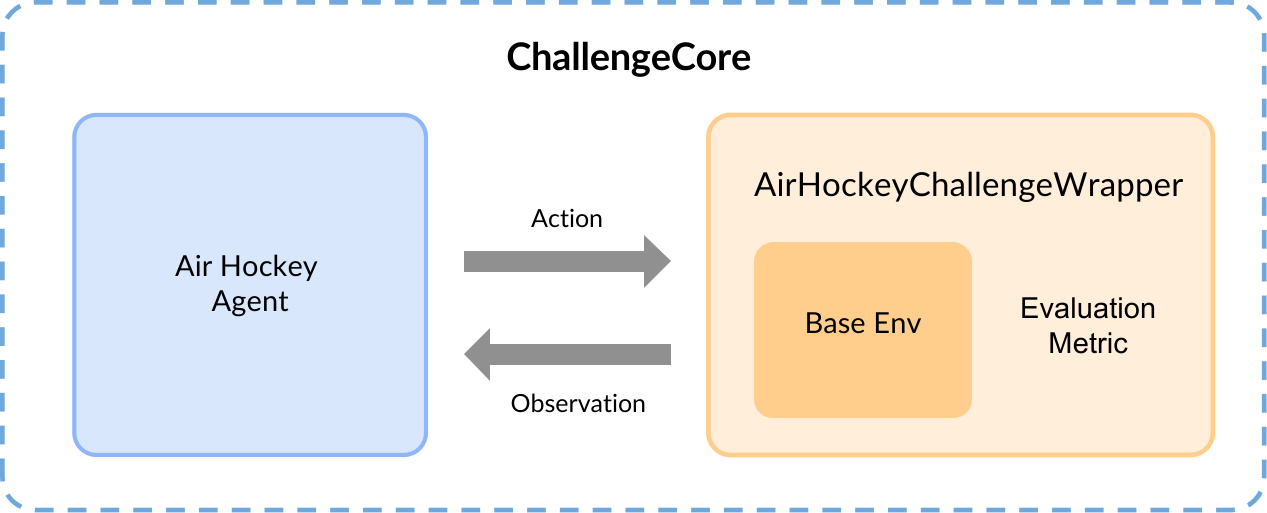
\includegraphics[width=0.8\textwidth]{Images/framework.png}
    \caption{Challenge framework.}
    \label{fig:framework}
\end{figure}

\subsection{Environments}
    The \textit{AirHockeyChallengeWrapper} component is a wrapper for the \textit{Base env} and processes the necessary information for the challenge evaluation.

    The simulated environment tries to mimic the real-world setup. The robot is controlled by a \textit{Tracking controller}, a Feedforward-PD controller, which sends 
    the torque command $\tau_{cmd}$ to the robot.

    \begin{equation*}
        \tau_{cmd} = M(q)\ddot{q}_d + c(q,\dot{q}) + g(q) + K_p(q_d - q) + K_d(\dot{q}_d - \dot{q})
    \end{equation*}

    The \textit{Trajectory interpolator}, by default a cubic polynomial, is used to interpolate the trajectory points between two consecutive commands.
    A \textit{Joint safety limiter} is used to avoid executing commands that exceed the position or velocity limits.

    \begin{figure}[H]
        \centering
        \label{fig:control_loop}
        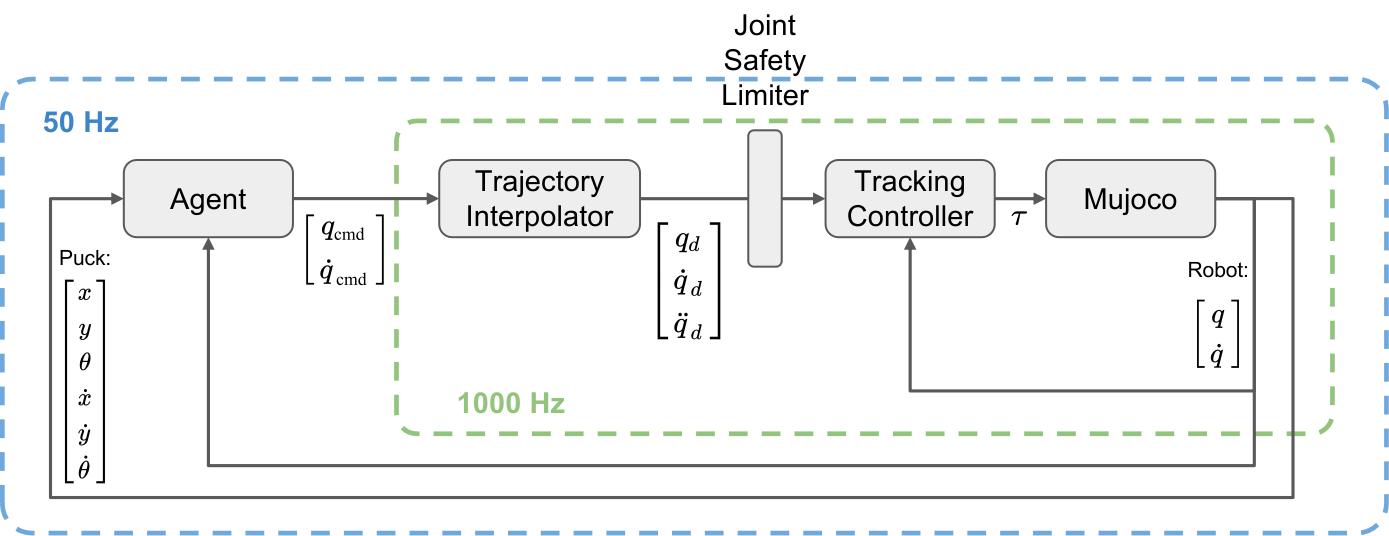
\includegraphics[width=0.8\textwidth]{Images/control_paradigm}
        \caption{Control loop.}

    \end{figure}

    %% Interpolation options

    The framework provides a flexible interface for commanding the robot in which the trajectory interpolation order can be specified:
    \begin{itemize}
        \item Cubic interpolation. The action command contains the desired [position, velocity]. A cubic polynomial is used to interpolate the intermediate steps.
        \item Linear interpolation. The action command contains the desired [position]. A linear polynomial is used to interpolate the intermediate steps.
        \item Quadratic interpolation. The action command contains the desired [position]. A quadratic function uses the previous position, velocity and the desired position to interpolate the intermediate steps.
        \item Quartic interpolation. The action command contains the desired [position, velocity]. A quartic function uses the previous position, velocity and the desired position, velocity to interpolate the intermediate steps.
        \item Quintic interpolation. The action command contains the desired [position, velocity, acceleration]. A quintic function is computed by the previous position, velocity, acceleration and the desired position, velocity and acceleration to interpolate the intermediate steps.
        \item Linear interpolation in position and velocity. The action command contains the desired [position, velocity]. The position and velocity will both be linearly interpolated. The acceleration is computed based on the derivative of the velocity. This interpolation is not proper, but it is useful to avoid oscillatory in the interpolation.
        \item None. The action can be a complete trajectory between each action step. At each step, the trajectory command should include desired [position, velocity, acceleration]
    \end{itemize}

    The air hockey table and its dimensions are illustrated in Figure \ref{fig:air_hockey_table}


    \begin{figure}[H]
        \centering
        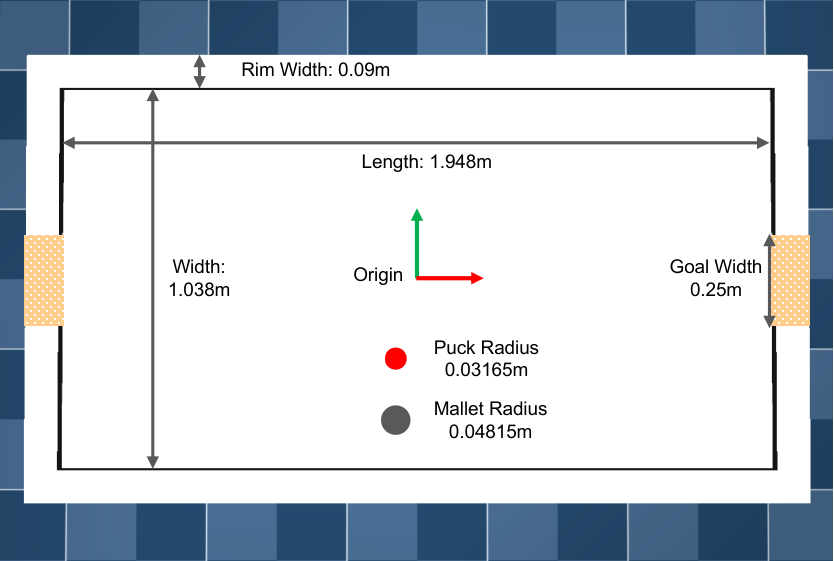
\includegraphics[width=0.8\textwidth]{Images/air_hockey_table}
        \caption{The air hockey table.}
        \label{fig:air_hockey_table}
    \end{figure}

\subsection{Robot models}
    \subsubsection{Planar robot - 3 degrees of freedom}
    During the Warm up stage the participants were provided a 3 DoF planar robot to understand how to use the framework.
    The robot is set such that the end-effector remains at the same height of the table surface. In simulation, the collision between the robot and the table are discarded.
    The base of the planar robot is located at [-1.51, 0., -0.1], the orientation is aligned with the world's frame, as illustrated in Figure \ref{fig:planar_env}


    Below the specification of the planar robot:
    \begin{itemize}
        \item \textbf{Position upper limit (rad)}: [ 2.967060, 1.8, 2.094395]
        \item \textbf{Position lower limit (rad)}: [-2.967060, -1.8, -2.094395]
        \item \textbf{Velocity limit (rad/s)}: +/- [1.570796, 1.570796, 2.094395]
        % \item \textbf{Link length (m)}: [0.55, 0.44, 0.44]
        \item \textbf{Initial position (rad)}: [-1.156, 1.300, 1.443]
        \item \textbf{Initial velocity (rad/s)} [0, 0, 0]
    \end{itemize}

    \subsubsection{KUKA iiwa14 LBR robot}
    The KUKA iiwa14 LBR robot is a general purpose manipulator with 7 degrees of freedom. A universal joint on the end-effector is added
    to increase the robot's flexibility. The universal joint is a passive joint that adapts the joint position based on contacts. In simulation, the collision between the robot and the table
    are discarded, requiring the agent to keep the mallet at an appropriate height.

    We define the End-Effector as the tip of the extension rod before the universal joint. 
    The end-effector's position can be fully determined by the robot's joint position and forward kinematics. 
    The base position of the robot is depicted in Figure \ref{fig:kuka_env}.

    Below the specification of the planar robot:
    \begin{itemize}
        \item \textbf{Position upper limit (rad)}: [ 2.967, 2.09 , 2.967, 2.094, 2.967, 2.094, 3.054]
        \item \textbf{Position lower limit (rad)}: [-2.967, -2.094, -2.967, -2.094, -2.967, -2.094, -3.054]
        \item \textbf{Velocity limit (rad/s)}: +/- [ 1.483, 1.483, 1.745, 1.308, 2.268, 2.356, 2.356]   
        \item \textbf{Initial position (rad)}: [ 0, -0.1960, 0, -1.8436, 0, 0.9704 0]
        \item \textbf{Initial velocity (rad/s)} [0, 0, 0, 0, 0, 0, 0]
    \end{itemize}


\subsection{Constraints}
To avoid losing points the robot must respect a set of constraints.
These constraints are described here:

\begin{itemize}
    \item \textit{JointPositionConstraint}: $q_l < q_{cmd} < q_u$
    \item \textit{JointVelocityConstraint}: $\dot{q}_l < \dot{q}_{cmd} < \dot{q}_u$
    \item \textit{EndEffectorConstraint}:
        \begin{equation*}
            \begin{aligned}
                & l_x < x_{ee} \\
                & l_y < y_{ee} < u_y \\
                & \text{table height} - \text{tolerance} < z_{ee} < \text{table height} + \text{tolerance}
            \end{aligned}
        \end{equation*}
    The End-Effector must not exceed the table and stay at
    \item \textit{LinkConstraint} (7 DoF Robot only):
    \begin{equation*}
        \begin{aligned}
            & z_{elbow} > 0.25 \\
            & z_{wrist} > 0.25
        \end{aligned}
    \end{equation*}
    \item \textit{ComputationTime}: The computation time at each step should be smaller than 0.02s.
\end{itemize}

\subsection{Evaluation Metrics}
    \begin{itemize}
        \item \textbf{Success Rate}:
        A success criterion is defined for each task. We will check if the task succeed when the episode terminates. Each episode can terminate because of two reasons: 1. maximum number of steps reached; 2. No further interaction can be in the episodes.
        \begin{itemize}
            \item Hit: The puck enters the scoring zone with a speed above the threshold.
            \item Defend: The final velocity of the puck (at the end of the game) is below the threshold and does not bounce to the other side of the court.
            \item Prepare: The final position of the puck is within a predefined area and at a speed less than the threshold.
        \end{itemize}

        \item \textbf{Deployability}: Each deployability metric is assigned one or multiple penalty points based on the level of risk. The deployability score is counted when the constraints of the evaluation metric are violated. Each metric is computed at most once per episode (maximum 500 steps per episode). 
        \begin{itemize}
            \item Violations of the End-Effector's Position Constraints (3 penalty points): 
            The desired x-y-position of the end-effector should remain within the boundaries of the table. The z-position of the end-effector should remain within a range.
            \item Violations of the Joint Position Limit Constraints (2 penalty points): The desired position command should not exceed the position limits.
            \item Violations of the Joint Velocity Limit Constraints (1 penalty point): The desired velocity command should not exceed the velocity limits.
            \item Computation Time (0.5-2 penalty points): The computation time at each step should be shorter than 0.02s.
        \end{itemize}
    \end{itemize}

    Each evaluation consisted of 1000 episodes. The success rates were used to rank the leaderboards. The deployability score is the sum of the penalty score from all episodes. The rankings were divided into three categories based on the score of deployability.
    \begin{enumerate}
        \item \textbf{Deployable}: $0 \le \text{deployability score} \le 500$
        \item \textbf{Improvable}: $500 < \text{deployability score} \le 1500$
        \item \textbf{Nondeployable}: $1500 < \text{deployability score}$
    \end{enumerate}

\subsection{Simulator}
    The simulator application of the Robot Air Hockey Challenge is summarized in the following:
    \begin{itemize}
        \item Simulator: MuJoCo \cite{MuJoCo}
        \item Simulation frequency: 1000 Hz
        \item Control Frequency: 50 Hz
        \item Observation:
            \begin{itemize}
                \item \textbf{Robot}:
                \begin{itemize}
                    \item Joint positions [radians]
                    \item Joint velocities [radians/s] computed by finite difference
                \end{itemize}
                \item \textbf{Puck} (relative to the robot base frame):
                    \begin{itemize}
                        \item X-Y position [m]
                        \item Yaw angle [radians]
                        \item X-Y velocity [m/s]
                        \item Yaw velocity [radians/s] computed by finite difference
                    \end{itemize}
                \item \textbf{Opponent} (if applicable)
                \begin{itemize}
                    \item End-effector-s X-Y position [m]
                \end{itemize}
            \end{itemize}
        \item Control action:
            \begin{itemize}
                \item We try to set the simulation as close as possible to the real-world setup. The robot is controlled by torque at 1000 Hz. We use a feed-forward + PD controller to determine the joint torque that tracks the desired joint position and velocity.
                \item A 20-step interpolation is required in the agent's adjacent control commands (the agent control frequency is 50 Hz). We provide different types of polynomial interpolation upon requirements. Details about the action interface can be found here.
            \end{itemize}
    \end{itemize}

